% $Header: /cvsroot/latex-beamer/latex-beamer/solutions/conference-talks/conference-ornate-20min.en.tex,v 1.6 2004/10/07 20:53:08 tantau Exp $

\documentclass[xcolor=x11names,table]{beamer}

%% \theoremstyle{plain} %% This is the default


% This file is a solution template for:

% - Talk at a conference/colloquium.
% - Talk length is about 20min.
% - Style is ornate.



% Copyright 2004 by Till Tantau <tantau@users.sourceforge.net>.
%
% In principle, this file can be redistributed and/or modified under
% the terms of the GNU Public License, version 2.
%
% However, this file is supposed to be a template to be modified
% for your own needs. For this reason, if you use this file as a
% template and not specifically distribute it as part of a another
% package/program, I grant the extra permission to freely copy and
% modify this file as you see fit and even to delete this copyright
% notice.

%% General document %%%%%%%%%%%%%%%%%%%%%%%%%%%%%%%%%%
\usepackage{pgf,pgfarrows,pgfnodes,pgfautomata,pgfheaps,pgfshade,sidecap}
\usepackage{graphicx}
\usepackage[english]{babel}
\usepackage{graphicx}
\usepackage{amsmath}
\usepackage{amsthm}
\usepackage{amssymb}
\usepackage{epstopdf}
\usepackage{bbm}
\usepackage{times}
\usepackage[T1]{fontenc}
\usepackage{amsfonts}
\usepackage{algorithm}
\usepackage{algorithmic}
%%%%%%%%%%%%%%%%%%%%%%%%%%%%%%%%%%%%%%%%%%%%%%%%%%%%%%

%
%\renewcommand{\(}{\begin{columns}}
%\renewcommand{\)}{\end{columns}}
%\newcommand{\<}[1]{\begin{column}{#1}}
%\renewcommand{\>}{\end{column}}
%%%%%%%%%%%%%%%%%%%%%

\mode<presentation> {
  \usetheme{Warsaw}
  \usefonttheme{professionalfonts}
  \usecolortheme{whale}
 \useoutertheme{infolines}
 \useinnertheme{rectangles}
  % or ...

  %\setbeamercovered{transparent}
  % or whatever (possibly just delete it)
}

% marcro definition
\newcommand{\bbr}{\mathbb{R}}  %black board bold \mathbb{R}
\newcommand{\bbn}{\mathbb{N}}
\newcommand{\bbp}{\mathbb{P}}
\newcommand{\bY}{\mathbf{Y}}
\newcommand{\mun}{\lceil \mu n \rceil}
\newcommand{\etan}{\lceil \eta n \rceil}
\newcommand{\bbq}{\mathbb{Q}}
\newcommand{\wQ}{\widetilde{\bbq}}
\newcommand{\wq}{\widetilde{q}}
\newcommand{\wY}{\widetilde{Y}}
\newcommand{\ow}{\overline{w}}
\newcommand{\wbY}{\widetilde{\bY}}
\newcommand{\D}{\mathbb{D}}
\newcommand{\G}{\mathbb{G}}
\newcommand{\bbe}{\mathbb{E}}
\newcommand{\F}{\mathbb{F}}
\newcommand{\HH}{\mathbb{H}}
\newcommand{\bbj}{\mathbb{J}}
\newcommand{\bbz}{\mathbb{Z}}
\newcommand{\bbs}{\mathbb{S}}
\newcommand{\C}{\mathbb{C}}
\newcommand{\bu}{\mathbf{u}}
\newcommand{\bx}{\mathbf{x}}
\newcommand{\fn}{\footnote}
\newcommand{\ci}{\citeasnoun}
\newcommand{\om}{\omega}
\newcommand{\la}{\lambda}
\newcommand{\tla}{\tilde{\lambda}}
\newcommand{\doth}{f}
%\renewcommand{\labelenumi}{\roman{enumi}}
\newcommand{\ps}{P}
\newcommand{\pss}{\ensuremath{\mathbf{p}}} %small boldface
\newcommand{\pmq}{\ensuremath{\mathbf{Q}}}
\newcommand{\pmqs}{\ensuremath{\mathbf{q}}}
\newcommand{\pas}{P-a.s. }
\newcommand{\pasm}{P\mbox{-a.s. }}
\newcommand{\asm}{\quad\mbox{a.s. }}
\newcommand{\cadlag}{c\`adl\`ag }
\newcommand{\fil}{\mathcal{F}}
\newcommand{\cF}{\mathcal{F}}
\newcommand{\gcal}{\mathcal{G}}
\newcommand{\hcal}{\mathcal{H}}
\newcommand{\jcal}{\mathcal{J}}
\newcommand{\pcal}{\mathcal{P}}
\newcommand{\ecal}{\mathcal{E}}
\newcommand{\bcal}{\mathcal{B}}
\newcommand{\ical}{\mathcal{I}}
\newcommand{\scal}{\mathcal{S}}
\newcommand{\ncal}{\mathcal{N}}
\newcommand{\lcal}{\mathcal{L}}
\newcommand{\kcal}{\mathcal{K}}
\newcommand{\acal}{\mathcal{A}}
\newcommand{\mcal}{\mathcal{M}}
\newcommand{\rcal}{\mathcal{R}}
\newcommand{\tcal}{\mathcal{T}}
\newcommand{\ti}{\times}
\newcommand{\we}{\wedge}
\newcommand{\be}{\begin{equation}}
\newcommand{\ee}{\end{equation}}
\newcommand{\bew}{\begin{equation*}}
\newcommand{\eew}{\end{equation*}}
\newcommand{\uK}{\underline K}
\newcommand{\oK}{\overline K}
\newcommand{\imp}{\eta}
\newcommand{\f}{\left}
\newcommand{\g}{\right}
\newcommand{\wht}{\widehat}
\newcommand{\wtd}{\widetilde}
\newcommand{\var}{Var}
\newcommand{\abs}[1]{\lvert#1\rvert}
\newcommand{\xbar}{\overline{X}}
\newcommand{\Xij}{X_{i,j}}
\newcommand{\naiveest}{\wht{\sigma^2_n}}
\newcommand{\deltaest}{\wht{\sigma^2_d}}

% or whatever


% or whatever


% try to modify left and upper border of whole presentation
%\geometry{left=1cm,top=1cm}
%\setbeamersize{sidebar width left=1cm, sidebar width right=1cm}
%\setbeamertemplate{headline}{\vspace{1cm}}
%\setbeamersize{text margin left=1cm, text margin right=1cm}

\title[Experiment Unit] % (optional, use only with long paper titles)
{Choice of Experiment Unit for Controlled Experiments on Web}


\author % (optional, use only with lots of authors)
{Shaojie Deng}

\addtobeamertemplate{title page}{}{\footnotesize \begin{center} Joint work with Roger Longbotham, Toby Walker and Ya Xu\end{center}}
% - Give the names in the same order as the appear in the paper.
% - Use the \inst{?} command only if the authors have different
%   affiliation.
%\addtobeamertemplate{title page}{}{\footnotesize \begin{center} Joint work with Hock Peng Chan (NUS), Shaojie Deng (Microsoft)\\ and Kay Giesecke (Stanford)\end{center}}
\institute[Microsoft] % (optional, but mostly needed)
{
  One Microsoft Way\\
  Microsoft
  }
% - Use the \inst command only if there are several affiliations.
% - Keep it simple, no one is interested in your street address.

\date{}
% - Either use conference name or its abbreviation.
% - Not really informative to the audience, more for people (including
%   yourself) who are reading the slides online

\subject{Controlled experiment on  web}
% This is only inserted into the PDF information catalog. Can be left
% out.
%\logo{\includegraphics[height=1cm,angle=90]{eisai.pdf}}

\AtBeginSection[] {
  \begin{frame}<beamer>
    \frametitle{Agenda}
\footnotesize
    \tableofcontents[currentsection]
  \end{frame}
}

\begin{document}

\begin{frame}  
  \titlepage
\end{frame}

\begin{frame}
  \frametitle{Outline}
\footnotesize
  \tableofcontents
  % You might wish to add the option [pausesections]
\end{frame}

\section{\scshape Introduction to Controlled Experiment on Web}
\begin{frame}{Introduction}
\footnotesize
\begin{columns}[t]
\column{2.8in}
\begin{itemize}
\item Controlled experiment or randomized experiment is the best-known scientific method for establishing causality between a feature and its effects.
\item The basic  methodology is to expose a percentage of users to a new treatment, measure the effect on metrics of interest, and run statistical tests to determine whether the differences are statistically significant, thus establish causality.
\item It is easy to collect data on web quickly and at low cost. Web provides an unprecedented opportunity for us to use the power of controlled experiment to test and evaluate ideas quickly.
\end{itemize}
\column{1.5in}
\begin{figure}[!htbp]
  \centering
  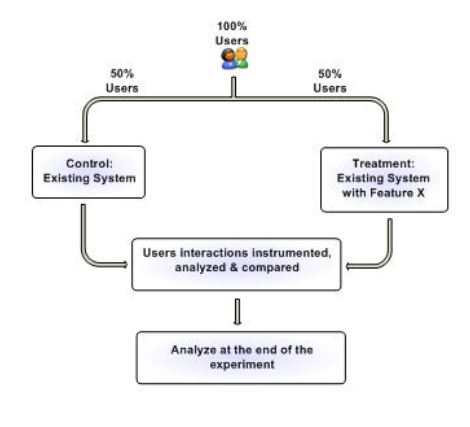
\includegraphics[width=1.2\textwidth]{split}
\end{figure}
\end{columns}
\end{frame}



\begin{frame}{Terminology}
\small
\begin{itemize}
\item {\bf Experiment Unit}: The unit on which the randomization is applied. Also called randomization unit. The most commonly used experiment unit is user or its surrogate such as cookie or user ID. Page view has also been used in practice.  
\pause
\item {\bf Metric}: An statistic stands for a concept that the experiment designer wants to evaluate. Common metrics include clicks per user, sessions per user, click through rate, coverage rate, revenue per user etc. 
\pause
\item {\bf Analysis Unit}: A metric is naturally associated with an analysis unit. For example, per user metric such as clicks per user has the analysis unit user. Click through rate and coverage rate use page view as the analysis unit. The analysis unit associated with a metric is also called the \emph{level} of the metric. The most important two types of metrics are user level metrics and page view level metrics.  
\pause
\item {\bf Measurement}: A measurement is an observation on an analysis unit. For example, the number of clicks of user $i$ on page view $j$ is a page view level measurement. It can be further rolled up (summed up) to user $i$'s total number of clicks, which is a user level measurement. 
\end{itemize}
\end{frame}

\begin{frame}
\begin{columns}[t]
\column{2in}
\begin{itemize}
\item Common experiment unit and analysis unit: user, page view
\item Analysis unit always finer than experiment unit. 
\item Interested in the following combinations:
\begin{enumerate}
\item E:User,A:User (Vanilla) 
\item E:User, A: Page View (Delta Method)
\item E:Page View, A: Page View (This Talk)	
\end{enumerate}
\end{itemize}
\column{2in}
\begin{figure}[!htbp]
  \centering
  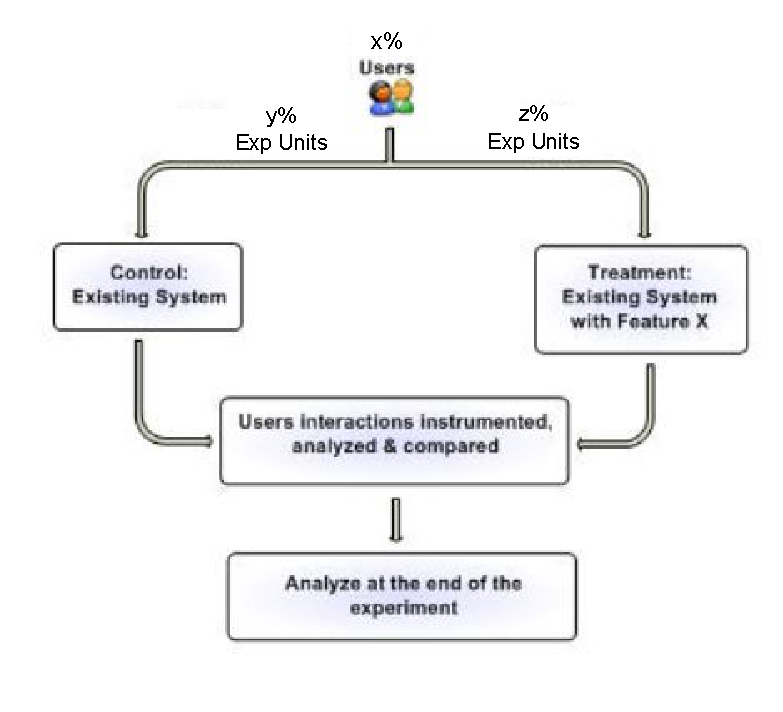
\includegraphics[width=1.2\textwidth]{split2}
\end{figure}
\end{columns}

\end{frame}

\begin{frame}{Two Sample T-test/Z-test}
\begin{itemize}
\item Given a metric $S$, we can calculate the value of this metric for both control group and treatment group, denoted by $S_c$ and $S_t$. We want to test whether $S_t-S_c=0$. 
\item Test statistics $\frac{S_t-S_c}{\sqrt{\var(S_t-S_c)}} =\frac{S_t-S_c}{\sqrt{\var (S_t-S_c)}}$. 
\item Central limit theorem guarantees that the test statistic is asymptotically normal. The crux of the problem is to estimate the variance of $S_t-S_c$.
\end{itemize}
\end{frame}


\section{User as the Experiment Unit}
\begin{frame}{Vanilla case: E: user+ A: user}
\begin{itemize}
\item Assume user i.i.d. sampled.  Hence user level measurements i.i.d.
\item $S_t$ and $S_c$ are sample means of user level measurements. 
\item Estimate variance of $S_t$ and $S_c$ by sample variance.
\item Since user i.i.d. and treatment and control have disjoint sets of users, $Var(S_t-S_c)=Var(S_t)+Var(S_c)$
\item Most widely used. Simple and easy to understand. 
\end{itemize}

\end{frame}

\begin{frame}{ E: user+ A: page view}
\begin{itemize}
\item $S_t$ and $S_c$ are sample means of page view level measurements. 
\item Common mistake is to treatment page view level measurements as i.i.d. Not true, because randomization was on user level, and there is strong between user variance. 
\item $Var(S_t)$ and $Var(S_c)$ can be estimated via delta method. 
\item Since user i.i.d. and treatment and control have disjoint sets of users, $Var(S_t-S_c)=Var(S_t)+Var(S_c)$. 
\item Widely used. But not always with delta method correctly applied. 
\end{itemize}
\end{frame}

\begin{frame}{Delta Method}
\begin{itemize}
\item Let $X_{i,j}$ be page level measurement for user-$i$'s $j^{th}$ page view, and $K_i$ be user-$i$'s number of page views.  User level measurement $(\sum_{i=1}^{K_i} X_{i,j}, K_i),i=1,\dots,n$ are i.i.d. Page view level metric is $\xbar=\frac{\sum_i \sum _j X_{i,j}}{\sum_i K_i}$.
\item  By letting $Y_i = \sum_{i=1}^{K_i} X_{i,j}$ and express $\xbar$ as $\sum_{i=1}^n Y_i / \sum_{i=1}^n K_i$, it is then a straightforward application of the delta method to get an asymptotically consistent estimator for $\var \xbar$:
\begin{align*}
\frac{1}{n} \Bigl\{ \frac{1}{\wht{\bbe K_i}^2}\wht{\var Y_i} + \frac{\wht{\bbe Y_i}^2}{\wht{\bbe K_i}^4}\wht{\var K_i} - 2\frac{\wht{\bbe Y_i}}{\wht{\bbe K_i}^3} \wht{Cov(Y_i,K_i)} \Bigr\} 
\end{align*}
where these ``hatted'' quantities are the sample mean, variance and covariance. 
\end{itemize}
\end{frame}


\section{Page view as the Experiment Unit}
\begin{frame}
\begin{itemize}
\item Cons: User level metrics not available; variance estimation not straightforward. User experience not consistent, limiting its adoption. 
\item Pros: Variance reduction for page view level metrics. Better statistical power. 
\item Page view randomization experiments are good for testing the effect of a treatment on page level metrics where consistent experience is not a requirement. For example, test performance metric such as page loading time, test certain ranking algorithm of a search engine, test conversion rate of a promotion page, etc...
\end{itemize}
\end{frame}

\begin{frame}{Variance of $S_t-S_c$?} 
\begin{itemize}
\item Remember that we only allocate $x\%$ users for page view level randomization experiments. 
\item Page views of these $x\%$ users are then split into treatment and control experience.
\item $Var(S_t)$ and $Var(S_C)$ can be estimated separately by delta method. But $S_t$ and $S_c$ are not independent and it is unclear how to compute $Var(S_t-S_c)$
\end{itemize}
\end{frame}


\begin{frame}{A Bottom-Up Probability Model}
\begin{itemize}
\item  Let $X_{i,j}^{(r)}$ be the page level measurement (e.g. number of clicks on the page) on user $i$'s $j^{th}$ page view in group $r$($r=1,2$ for control and treatment).
\item $X_{i,j}^{(r)}$  has mean $\mu_i$ and variance $\sigma_i^2$ where $(\mu_i, \sigma_i^2)$ can differ from user to user but is fixed for each user. We call this the user effect. Under null hypothesis, control and treatment are the same and we assume $(\mu_i, \sigma_i^2)$ follows the same distribution.
\item $K_i$ the total number of page views from user $i$ and $N = \sum_{i=1}^n K_i$ be the total number of page views. Each $K_i$ are splitted into control and treatment, with $K_i^{(1)}$ and $K_i^{(2)}$ for each group. Let $N_{r}, r=1,2$ be total number of page views. 
\item Assume $K_i,i=1,\dots,n$ are i.i.d. and independent of $(\mu_i,\sigma_i^2),i=1,\dots,n$.(Not always true, need to check this assumption case by case.) 
\end{itemize}
\end{frame}

%\begin{frame}{Road Map}
%\small
%\begin{itemize}
%\item $S_t = \xbar_2$, $S_c=\xbar_1$.
%\item Let
%$
%\naiveest_r = n\times \frac{1}{N_r^2} \Bigl (\sum_{i=1}^n \sum_{j=1}^{K_i^{(r)}} (X_{i,j}^{(r)}-\overline{X})^2 \Bigr )
%$ ,
%$
%\deltaest_r =  \Bigl\{ \frac{1}{\wht{\bbe K_i^{(r)}}^2}\wht{\var Y_i^{(r)}} + \frac{\wht{\bbe Y_i^{(r)}}^2}{\wht{\bbe K_i^{(r)}}^4}\wht{\var K_i^{(r)}} - 2\frac{\wht{\bbe Y_i^{(r)}}}{\wht{\bbe K_i^{(r)}}^3} \wht{Cov(Y_i^{(r)},K_i^{(r)})} \Bigr\} 
%$
%\item We give a consistent estimator of $\var(\xbar_2-\xbar_1)$.
%\item We verify the formula with simulation. 
%\end{itemize}
%\end{frame}

\begin{frame}{Road Map}
\small
\begin{itemize}
\item $S_t = \xbar_2$, $S_c=\xbar_1$.
\item For asmyptotic analysis, \\
let $\naiveest_r$ = $n\times$ naive estimator of $\var \xbar_r$.\\
$\deltaest_r $=  $n\times$ delta method estimator of  $\var \xbar_r$.
\item We give a consistent estimator of $n\var(\xbar_2-\xbar_1)$.
\item We verify the formula with simulation. 
\end{itemize}
\end{frame}

\begin{frame}
\small
\begin{theorem}
Let $C_r = \bbe[ (K_i^{(r)})^2] / (\bbe K_i^{(r)})^2,r=1,2$, $C_x = \bbe (K_i^{(1)}K_i^{(2)})/(\bbe K_i^{(1)}\bbe K_i^{(2)})$. As $n\to \infty$. 
\begin{align*}
\naiveest_r &\to  \frac{1}{\bbe(K_i^{(r)})} (\var(\mu_i)+\bbe(\sigma_i^2)). \\
\deltaest_r &\to C_r \var(\mu_i) + \bbe(\sigma^2_i)/\bbe (K_i^{(r)}).\\
  n\var(\xbar_2-\xbar_1) &\to (C_1+C_2-2C_x) \var(\mu_i) + \Biggl(\frac{1}{\bbe K_i^{(1)}}+\frac{1}{\bbe K_i^{(2)}}\Biggr )\bbe(\sigma^2_i).
\end{align*}
Moreover, $C_1+C_2-2C_x= \frac{1}{\bbe K_i^{(1)}}+\frac{1}{\bbe K_i^{(2)}}$ . Therefore
\begin{align*}
n\var(\xbar_2-\xbar_1) \to\Biggl(\frac{1 }{\bbe K_i^{(1)}}+\frac{1}{\bbe K_i^{(2)}}\Biggr) \Bigl( \var \mu_i + \bbe \sigma_i^2\Bigr).
\end{align*}
i.e., \alert{ $\naiveest_1+\naiveest_2 \to n\var(\xbar_2-\xbar_1)$  \quad (Formula X)}.
\end{theorem}
\end{frame}

\begin{frame}
\begin{itemize}
\item  $n\var(\xbar_1)$ and $n\var (\xbar_2)$ should be estimated by delta method estimator $\deltaest_1$ and $\deltaest_2$, respectively.
\item But $n\var(\xbar_2-\xbar_1)$ can be consistently estimated by sum of two naive estimators as if treating page view level measurements i.i.d. 
\item Intuition is that if no user effect, i.e., $\mu_i,\sigma_i^2$ are the same for all users, we can treat page view level measurements i.i.d.
\item When page view used as experiment unit, user effect are essentially randomized. 
\item Empirical data suggest the variance between user $\var \mu_i$ are usually larger than within user variance $\bbe \sigma_i^2$. This means $\deltaest$ much larger than $\naiveest$. Therefore with page view as experiment unit, variance of $S_t-S_c$ are reduced comparing to user as experiment unit.
\end{itemize}
\end{frame}


\begin{frame}{Simulation Results: Page click rate}
N=1,000,000 users. User page click rate $\mu_i$ from $Beta(0.1,0.5)$. Sessions of each user from Poisson(2), then Page view for each session Poisson(3).  100,000 simulation runs. 95\% CI for true variance from 100 bootstraps. 
\begin{figure}[!htbp]
  \centering
  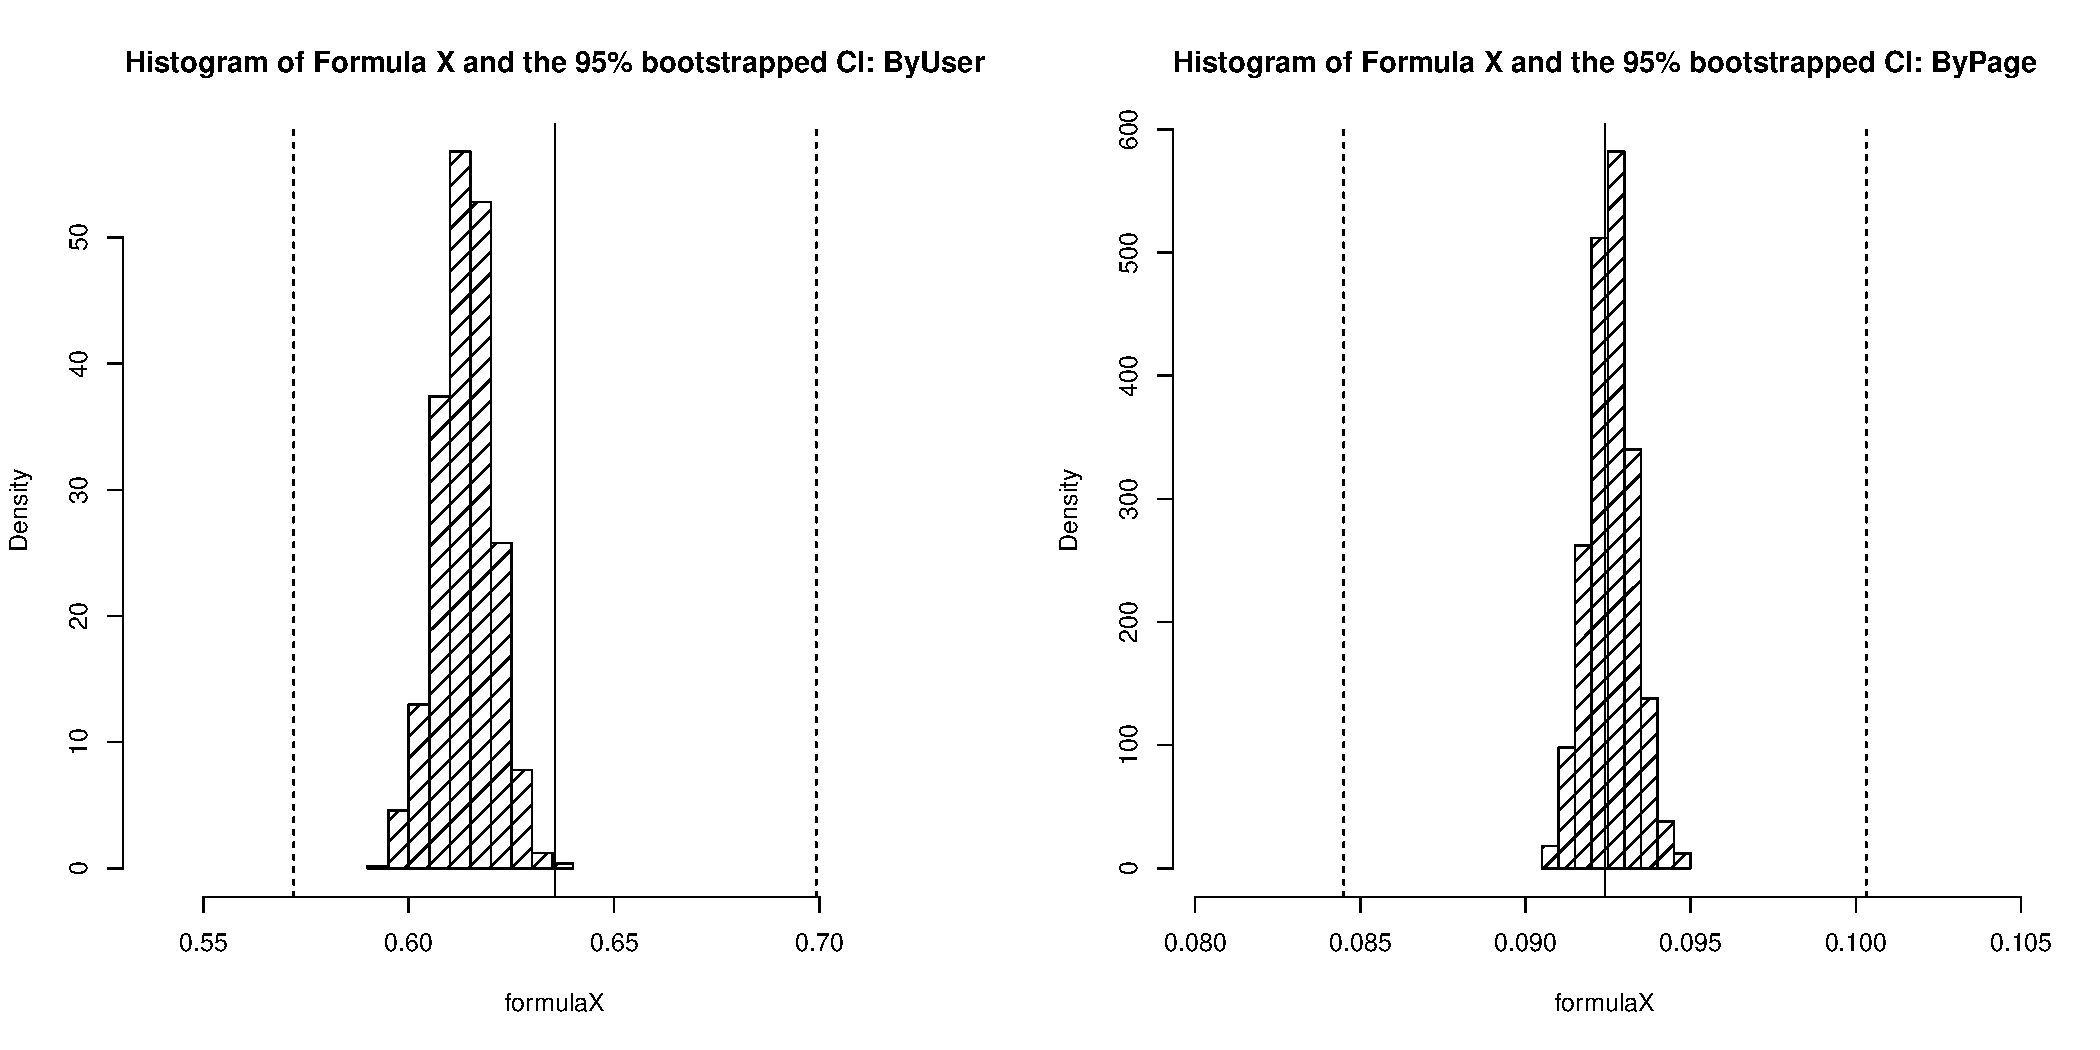
\includegraphics[width=1\textwidth]{jsm}
\end{figure}
\end{frame}



\section{\scshape Conclusion and Future Work }
\begin{frame}
\begin{itemize}
\item We presented a solution for statistical testing in the case of page view as both experiment and analysis unit.
\item Simulation result shows the performance of the formula X for variance estimation.
\item Simulation result shows for the same page view level metrics, using page view as experiment unit leads to much smaller variance.
\item We can use other units such as user session (visit) as experiment unit. Using session as both advantage of variance reduction and yet provide reasonable user experience consistency.  Formula X can be easily extended. 
\end{itemize}
\end{frame}
 

   
\section{Other Experiment Unit(Internal Review)}
\begin{frame}
\begin{itemize}
\item  $n\var(\xbar_1-\xbar_2) \to (C_1+C_2-2C_x) \var(\mu_i) + \Biggl(\frac{1}{\bbe K_i^{(1)}}+\frac{1}{\bbe K_i^{(2)}}\Biggr )\bbe(\sigma^2_i)$ works as long as the assumption $K_i$ independent of $(\mu_i,\sigma_i^2)$ is valid. \alert{ It does not depends on the choice of experiment unit}.
\item  However, $C_1+C_2-2C_x= \frac{1}{\bbe K_i^{(1)}}+\frac{1}{\bbe K_i^{(2)}}$ requires experiment unit to be page view.
\item Using $\naiveest_1$ and $\deltaest_1$, we  can solve $\var(\mu_i)$ and $\bbe(\sigma_i^2)$. We then could plug them into $(C_1+C_2-2C_x) \var(\mu_i) + \Biggl(\frac{1}{\bbe K_i^{(1)}}+\frac{1}{\bbe K_i^{(2)}}\Biggr )\bbe(\sigma^2_i)$ to get a consistent estimator for $\var(\xbar_1-\xbar_2)$.
\item In particular, if randomize by user, $C_x=0$ since one of $K_i^{(1)}$ and $K_i^{(2)}$ is 0. The formula above reduces to sum of two variance estimations vis the delta method.
\item In general, $C_x>0$ when experiment unit is finer than user. The finer the experiment unit, the smaller $C_1+C_2-C_x$ will be. 
\end{itemize}
\end{frame}
 
  \begin{frame}{Simulation}
\begin{figure}[!htbp]
  \centering
  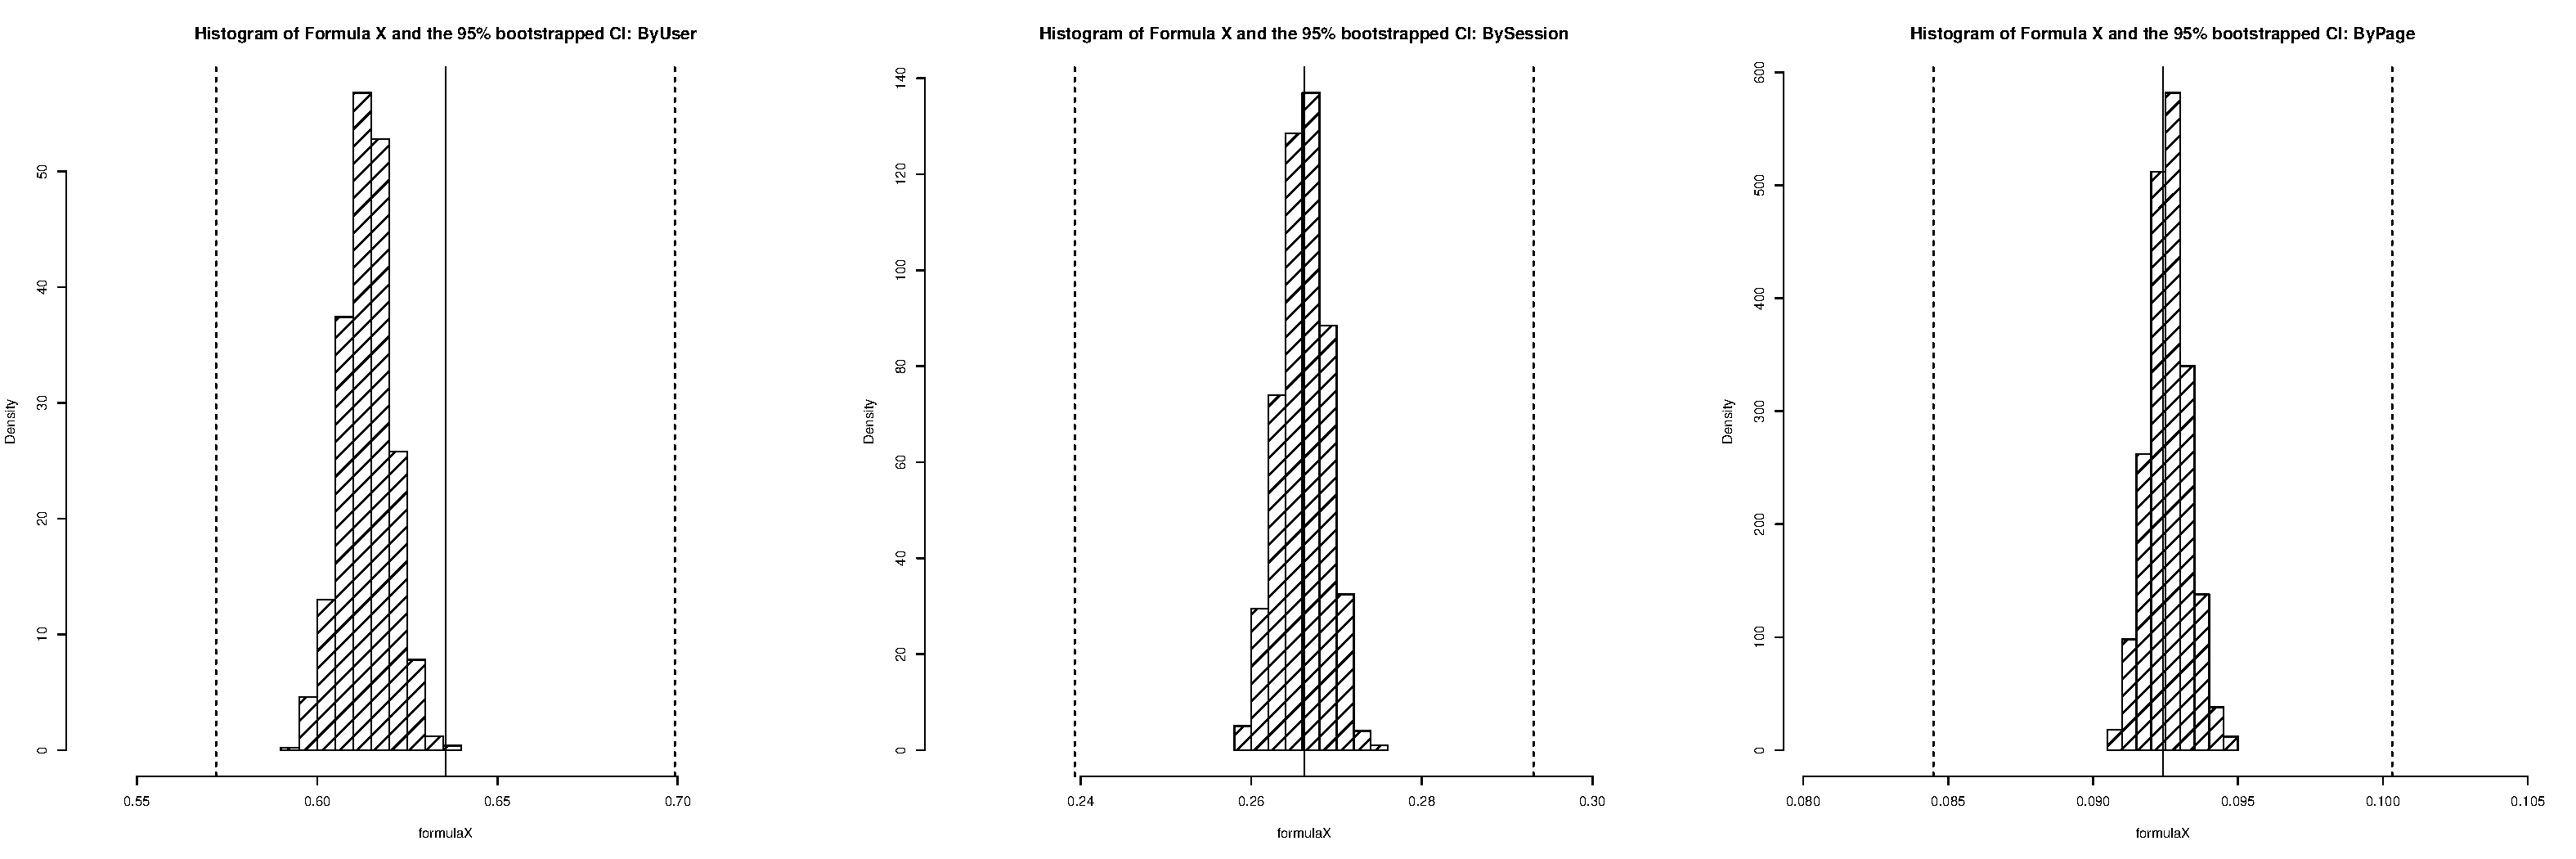
\includegraphics[width=1\textwidth]{jsm2}
\end{figure}
\end{frame}
 
  \begin{frame}{Fair Pair Experiment}
\begin{itemize}
\item  Reid Anderson's team did a randomization by query+user experiment. i.e.same MUID and same query will always get the same treatment. Control and treatment ratio is 3:1. Total 570,880 users with 3,448,247 page views.
\item Treatment  shifts answer insertion downward by 1 position.
\item Variance of win rate from 1,000 bootstrap : 0.0541.(Surrogate of the true variance)
\item Variance of win rate from Formula X: 0.0569.
\item If used user as experiment unit, variance would be 0.1124. 
\end{itemize}
\end{frame}
 

  
 

\end{document}

\section{Other Experiment Unit(Internal Review)}
\begin{frame}
\begin{itemize}
\item  $n\var(\xbar_1-\xbar_2) \to (C_1+C_2-2C_x) \var(\mu_i) + \Biggl(\frac{1}{\bbe K_i^{(1)}}+\frac{1}{\bbe K_i^{(2)}}\Biggr )\bbe(\sigma^2_i)$ works as long as the assumption $K_i$ independent of $(\mu_i,\sigma_i^2)$ is valid. \alert{ It does not depends on the choice of experiment unit}.
\item  However, $C_1+C_2-2C_x= \frac{1}{\bbe K_i^{(1)}}+\frac{1}{\bbe K_i^{(2)}}$ requires experiment unit to be page view.
\item Using $\naiveest_1$ and $\deltaest_1$, we  can solve $\var(\mu_i)$ and $\bbe(\sigma_i^2)$. We then could plug them into $(C_1+C_2-2C_x) \var(\mu_i) + \Biggl(\frac{1}{\bbe K_i^{(1)}}+\frac{1}{\bbe K_i^{(2)}}\Biggr )\bbe(\sigma^2_i)$ to get a consistent estimator for $\var(\xbar_1-\xbar_2)$.
\item In particular, if randomize by user, $C_x=0$ since one of $K_i^{(1)}$ and $K_i^{(2)}$ is 0. The formula above reduces to sum of two variance estimations vis the delta method.
\item In general, $C_x>0$ when experiment unit is finer than user. The finer the experiment unit, the smaller $C_1+C_2-C_x$ will be. 
\end{itemize}
\end{frame}
 
  \begin{frame}{Simulation}
\begin{figure}[!htbp]
  \centering
  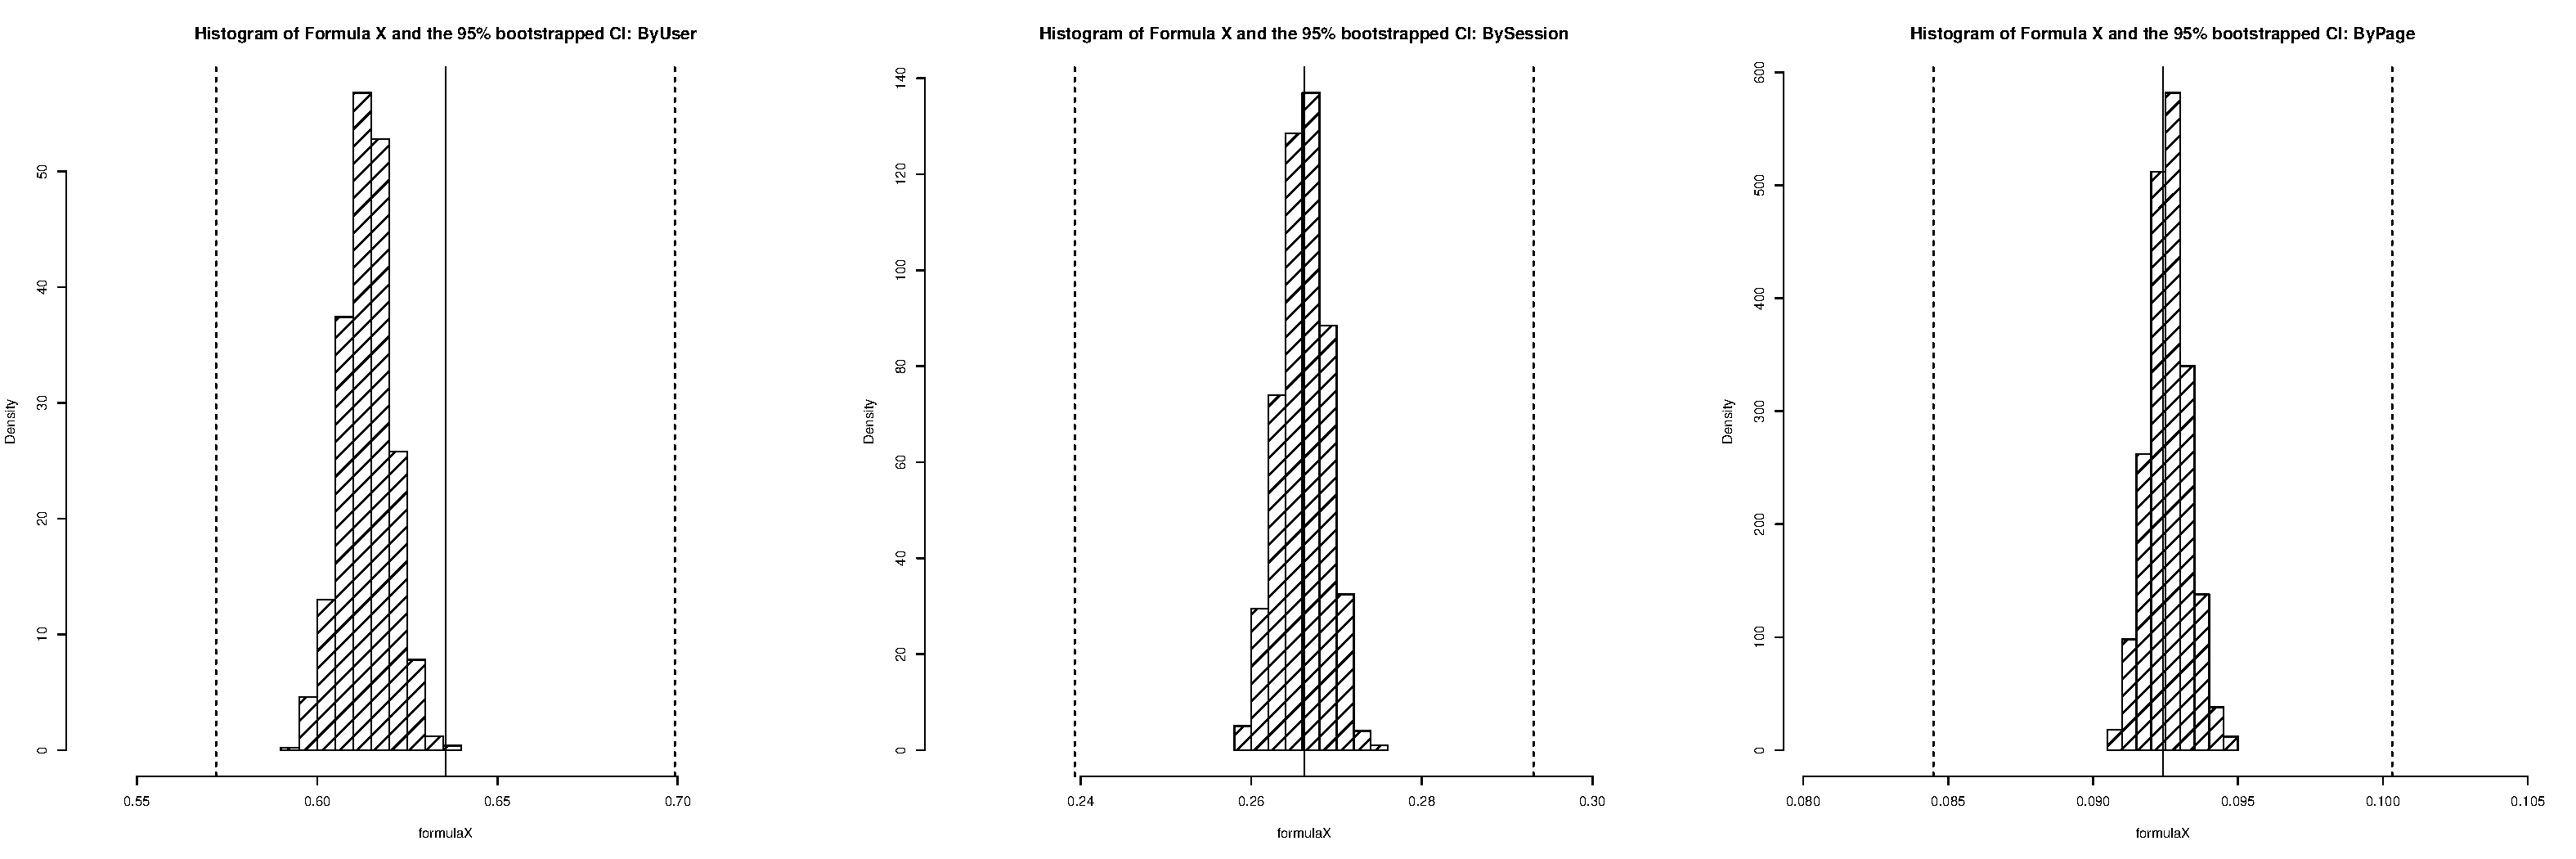
\includegraphics[width=1\textwidth]{jsm2}
\end{figure}
\end{frame}
 
  \begin{frame}{Fair Pair Experiment}
\begin{itemize}
\item  Reid Anderson's team did a randomization by query+user experiment. i.e.same MUID and same query will always get the same treatment. Control and treatment ratio is 3:1. Total 570,880 users with 3,448,247 page views.
\item Treatment  shifts answer insertion downward by 1 position.
\item Variance of win rate from 1,000 bootstrap : 0.0541.(Surrogate of the true variance)
\item Variance of win rate from Formula X: 0.0569.
\item If used user as experiment unit, variance would be 0.1124. 
\end{itemize}
\end{frame}